% Gemini theme, https://github.com/anishathalye/gemini
\documentclass[final]{beamer}

% ====================
% Packages
% ====================

\usepackage[T1]{fontenc}
\usepackage{lmodern}
\usepackage[size=custom,width=118.9,height=84.1,scale=1.15]{beamerposter}
\usetheme{gemini}
\usecolortheme{ENSA}
\usepackage{graphicx}
\usepackage{booktabs}
\usepackage{tikz}
\usepackage{pgfplots}
\pgfplotsset{compat=1.14}
\usepackage{anyfontsize}
\usepackage{hyperref}
\hypersetup{pdftitle={From Simulated Falls to Freezing of Gait: A Controlled Study of Domain Shift in Wearable Accelerometry},pdfauthor={Paul Christopher Aime}}
\graphicspath{{../../results/figures/}}

% ====================
% Lengths
% ====================

\newlength{\sepwidth}
\newlength{\colwidth}
\setlength{\sepwidth}{0.025\paperwidth}
\setlength{\colwidth}{0.3\paperwidth}

\newcommand{\separatorcolumn}{\begin{column}{\sepwidth}\end{column}}

% ====================
% Title
% ====================

\title{From Simulated Falls to Freezing of Gait: A Controlled Study of Domain Shift in Wearable Accelerometry}

\author{Paul Christopher Aim\'e \and Supervisor: Pr.\ Mustapha Ameur}

\institute[shortinst]{\'Ecole Nationale des Sciences Appliqu\'ees de Marrakech, Cadi Ayyad University, Morocco}

% ====================
% Footer
% ====================

\footercontent{
  Department of Computer Engineering \hfill
  Code, notebooks and checkpoints: \texttt{parkinson-domain-shift} repository \hfill
  \href{mailto:paulchristaimeslg3@gmail.com}{paulchristaimeslg3@gmail.com}}

% ====================
% Body
% ====================

\AtEndDocument{\directlua{pdf.setinfo('/Author (Paul Christopher Aime)')}}
\begin{document}

\begin{frame}[t]
\hypersetup{pdfauthor={Paul Christopher Aime}}
\begin{columns}[t]
\separatorcolumn

% ------------------------------------------------------------------ column 1
\begin{column}{\colwidth}

  \begin{block}{Question}
    Wearable fall detectors are trained on healthy volunteers who simulate falls on mattresses.
    Patients with Parkinson's disease rarely fall that way: many falls start with
    \textbf{freezing of gait (FoG)}, a brief inability to step. We ask whether a deep fall
    detector trained on \textbf{SisFall} (38 healthy subjects) can flag FoG in \textbf{Daphnet}
    (10 Parkinson's patients) without any patient label, and if not, \emph{why not}.
    \begin{itemize}
      \item \textbf{covariate shift}: normal movement differs (age, pathology);
      \item \textbf{concept shift}: the event to detect is a different phenomenon.
    \end{itemize}
  \end{block}

  \begin{block}{A controlled comparison}
    Sensor placement, units, labelling and training regime can all masquerade as ``domain shift''.
    Each is removed by construction:
    \begin{itemize}
      \item one accelerometer at the same site (waist / lower trunk), rotated into a
            vertical--antero-posterior--medio-lateral frame identified from the data;
      \item both domains in $g$ at 64\,Hz (SisFall downsampled with anti-aliasing);
      \item fall labels centred on the detected impact instead of the whole file;
      \item identical seeds, mini-batches, loss, optimiser and tuning budget for all four models.
    \end{itemize}
    \begin{figure}
      \centering
      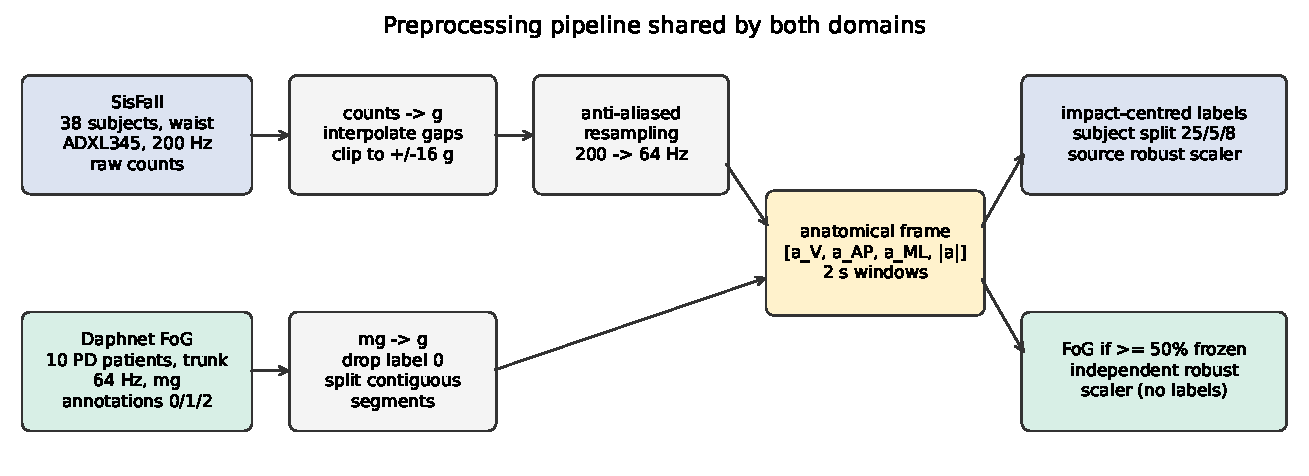
\includegraphics[width=\linewidth]{fig01_pipeline}
    \end{figure}
  \end{block}

  \begin{block}{What changes between the domains}
    \begin{figure}
      \centering
      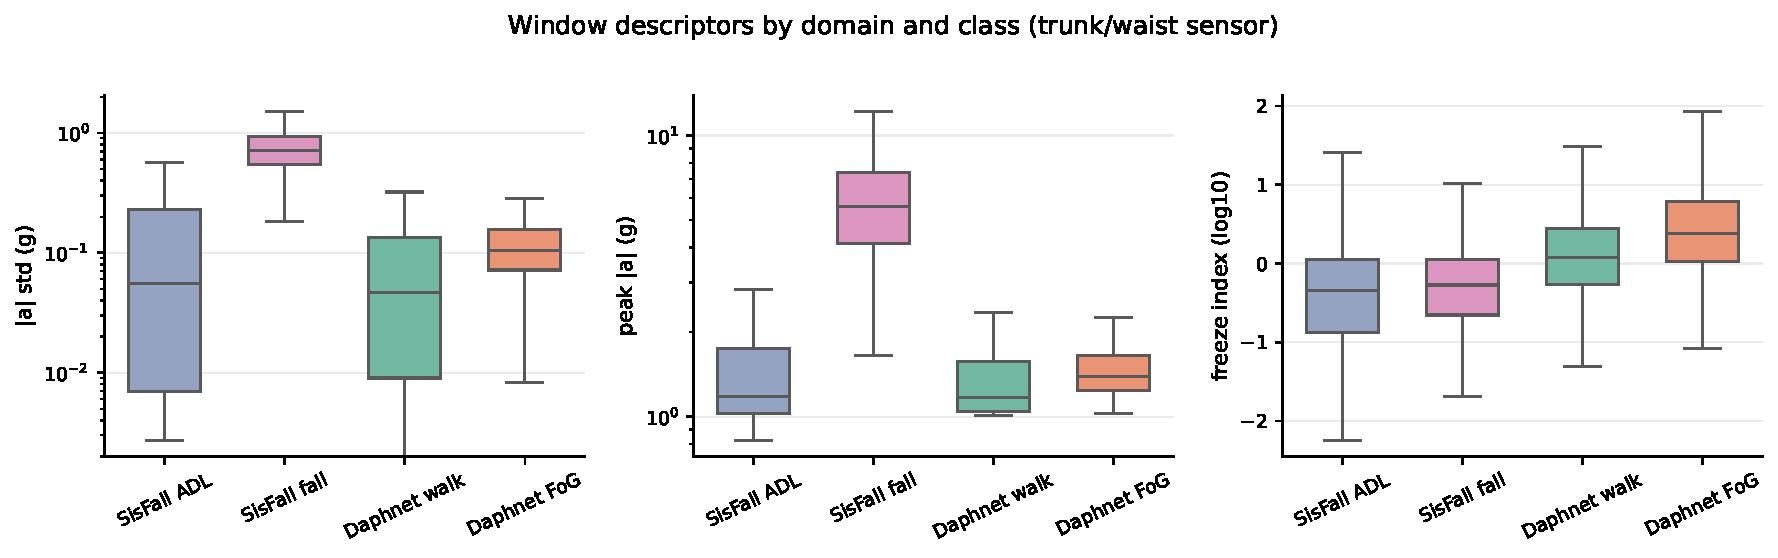
\includegraphics[width=\linewidth]{fig06_window_descriptors}
      \caption{A fall window peaks at $5.6\,g$. A FoG window differs from Parkinsonian walking by
      only $0.2\,g$ in peak, twice the $|a|$ variability and more power in the 3--8\,Hz freeze band.}
    \end{figure}
  \end{block}

\end{column}

\separatorcolumn

% ------------------------------------------------------------------ column 2
\begin{column}{\colwidth}

  \begin{block}{Models}
    \begin{tabular}{lrl}
\toprule
Model & Params & Selected configuration \\
\midrule
CNN-1D & 36k & 3 conv blocks (32--64--128), global avg.\ pooling \\
LSTM & 135k & 2 layers, bidirectional, hidden 64 \\
GRU & 26k & 2 layers, bidirectional, hidden 32 \\
Transformer & 70k & 16 patches of 0.125\,s, $d{=}64$, 2 layers, [CLS] \\
\bottomrule
\end{tabular}

\vspace{0.6ex}
\small 2\,s windows of $[a_V, a_{AP}, a_{ML}, |a|]$, robust scaling, weighted BCE, AdamW, 3 seeds,
equal tuning budget; threshold chosen on SisFall validation ($F_2$).

  \end{block}

  \begin{alertblock}{Main result}
    \begin{tabular}{lcccc}
\toprule
 & \multicolumn{2}{c}{SisFall test} & \multicolumn{2}{c}{Daphnet zero-shot} \\
\cmidrule(lr){2-3}\cmidrule(lr){4-5}
Model & AUROC & false alarms/h & AUROC & FoG recall \\
\midrule
CNN-1D & 0.988 & 1.5 & 0.49 & 0.9\% \\
LSTM & \textbf{0.999} & 0.8 & 0.59 & 0.1\% \\
GRU & \textbf{0.999} & \textbf{0.7} & \textbf{0.63} & 0.0\% \\
Transformer & 0.998 & 0.9 & 0.62 & 0.0\% \\
\midrule
Freeze index (no training) & -- & -- & \textbf{0.66} & -- \\
\bottomrule
\end{tabular}

\vspace{0.8ex}
Near-perfect fall detectors become \textbf{blind to freezing}: they rank FoG barely above
chance and stay silent at their validated threshold, while false alarms on Parkinsonian walking rise
\textbf{15--18$\times$}. Only the Transformer's patient-level 95\% CI excludes chance
(seed ensemble 0.65 [0.55, 0.73]).

  \end{alertblock}

  \begin{block}{In-domain vs.\ zero-shot}
    \begin{figure}
      \centering
      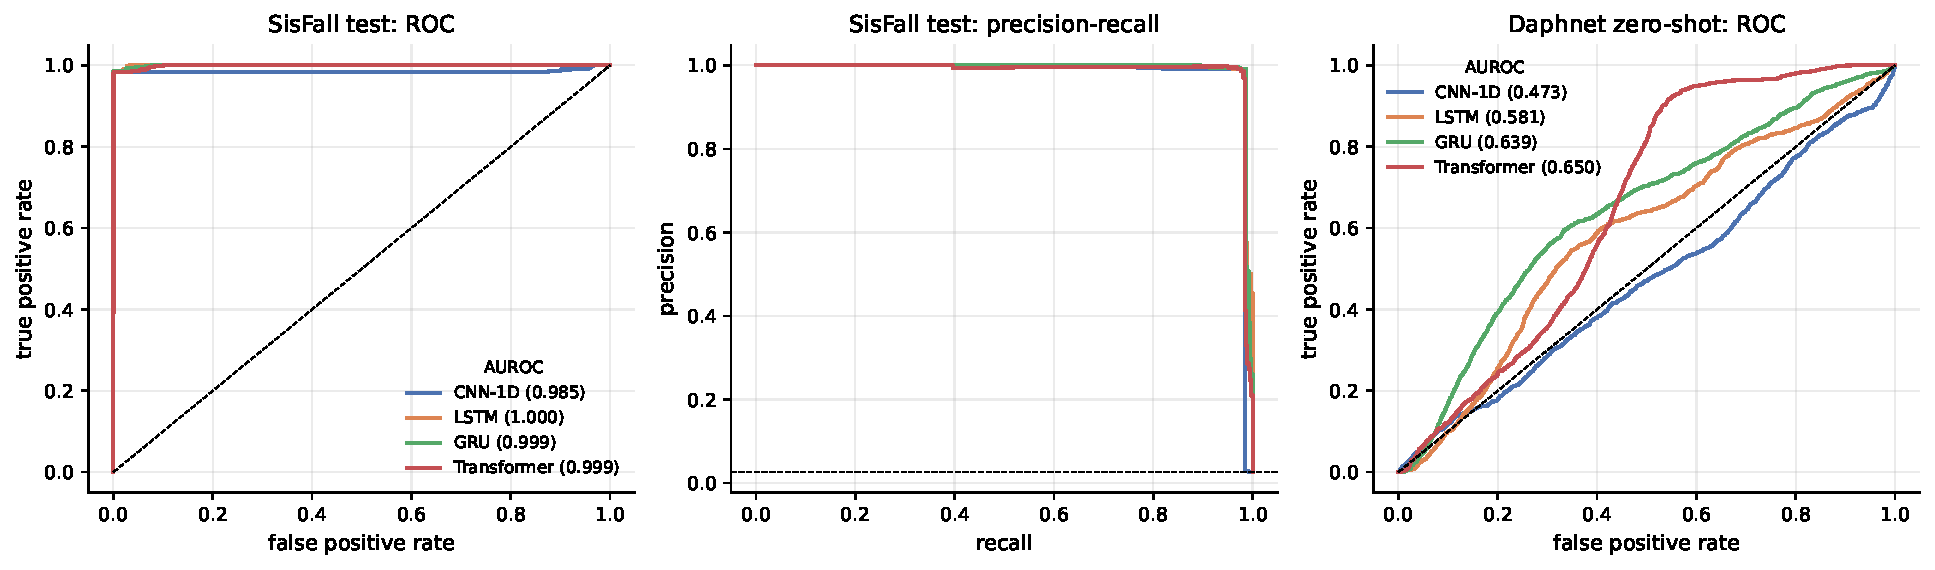
\includegraphics[width=\linewidth]{fig14_roc_pr_curves}
      \caption{Seed-averaged ROC / PR curves. Left, centre: SisFall test subjects. Right: Daphnet.}
    \end{figure}
  \end{block}

  \begin{block}{References}
    \scriptsize
    Sucerquia et al., SisFall, \emph{Sensors} 2017 \textbullet{}
    B\"achlin et al., Daphnet, \emph{IEEE TITB} 2010 \textbullet{}
    Moore et al., freeze index, \emph{J.\ Neurosci.\ Methods} 2008 \textbullet{}
    Nie et al., PatchTST, ICLR 2023 \textbullet{}
    Gulrajani \& Lopez-Paz, DomainBed, ICLR 2021 \textbullet{}
    Ben-David et al., \emph{Machine Learning} 2010 \textbullet{}
    Gretton et al., MMD, \emph{JMLR} 2012.
  \end{block}

\end{column}

\separatorcolumn

% ------------------------------------------------------------------ column 3
\begin{column}{\colwidth}

  \begin{block}{Why transfer fails}
    \begin{figure}
      \centering
      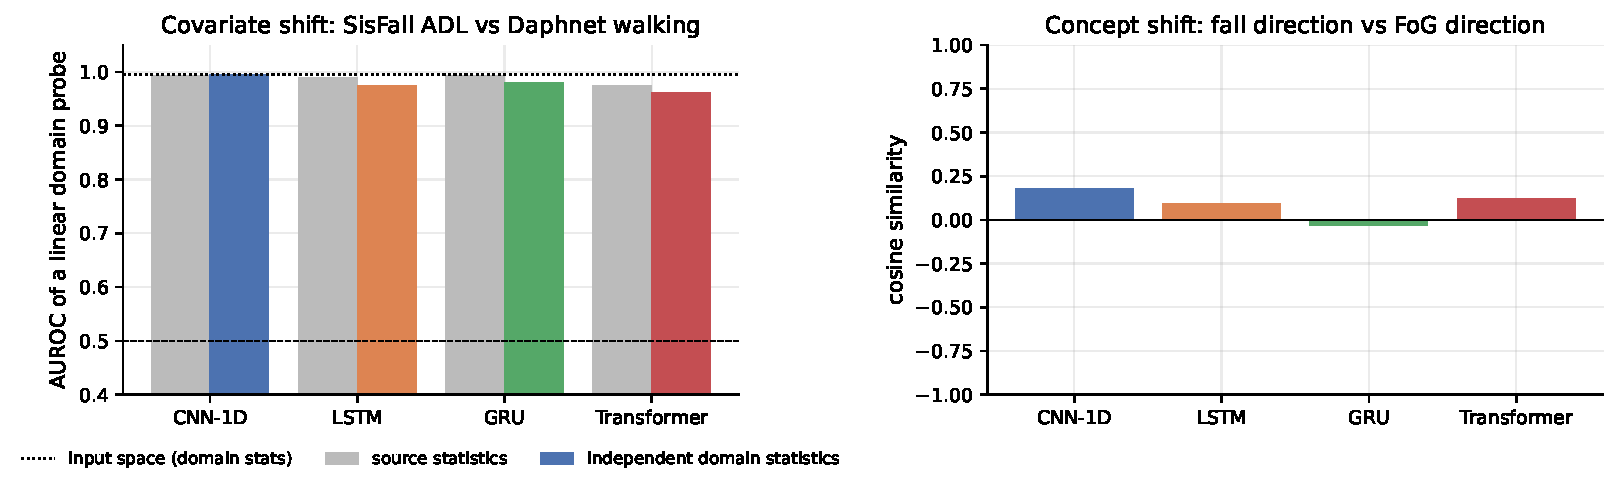
\includegraphics[width=\linewidth]{fig21_shift_decomposition}
    \end{figure}
    \begin{itemize}
  \item \textbf{Covariate shift persists.} A linear probe separates healthy ADL from Parkinsonian walking in every
        embedding (AUROC 0.96--0.995). Re-normalising Daphnet changes zero-shot AUROC by at most
        $\pm$0.13, with no consistent gain.
  \item \textbf{Concept shift dominates.} In raw statistics, FoG and falls both mean ``more movement''
        ($\cos = 0.77$). In the learned embeddings the fall direction is nearly orthogonal to the FoG
        direction ($\cos = -0.03$ to $0.18$): the networks learned impacts, not agitation.
  \item \textbf{Negative transfer.} Fine-tuning from fall weights is worse than training from scratch
        for all four models with 6 labelled patients (AUROC $-0.04$ to $-0.17$).
\end{itemize}

  \end{block}

  \begin{block}{Where each model stands}
    \begin{figure}
      \centering
      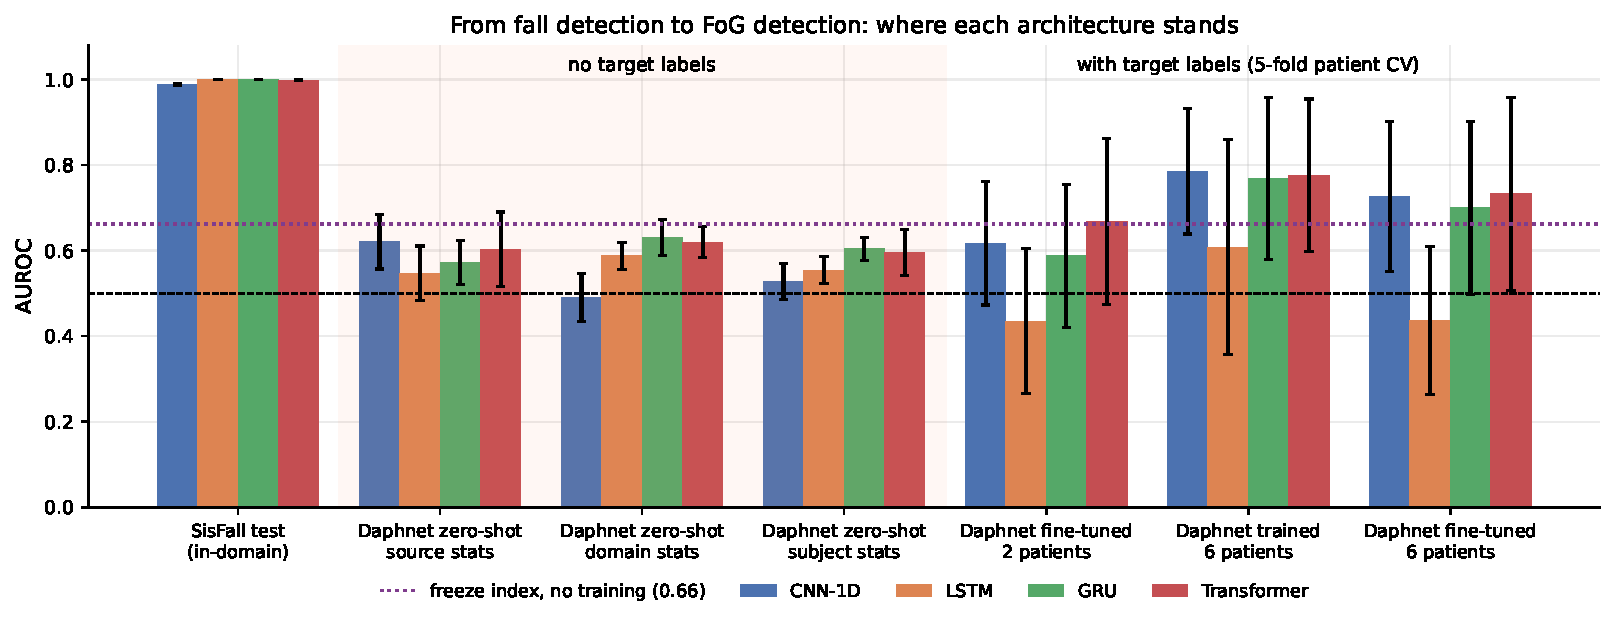
\includegraphics[width=\linewidth]{fig22_overview_auroc}
    \end{figure}
  \end{block}

  \begin{block}{Take-aways}
    \begin{enumerate}
  \item In-domain accuracy (AUROC $\approx$ 0.99 for every model) says nothing about transfer, and
        source validation cannot rank models by transferability.
  \item With matched sensors and impact-centred labels, the detectors are specific to impacts, not to
        ``abnormal movement'': they stay silent on freezing.
  \item The gap is a change of event, not only of population: physics-based features or
        event-agnostic self-supervised pre-training are better starting points than fall labels.
  \item With 6 labelled patients a trunk sensor reaches AUROC $\approx$ 0.78 (CNN-1D, Transformer,
        GRU), the realistic ceiling for this setting.
\end{enumerate}

  \end{block}



\end{column}

\separatorcolumn
\end{columns}
\end{frame}

\end{document}
